\documentclass{article}
\usepackage[utf8]{inputenc}


% TEMPLATE COMMENTS FORMATTING
\usepackage{amsmath,amssymb}
\usepackage{ifthen}
\usepackage[dvipsnames]{xcolor}
\usepackage[most]{tcolorbox}
\usepackage{soul}
\usepackage{listings}
\usepackage[T1]{fontenc}
\usepackage{hyperref}
\usepackage{subcaption}
\usepackage{adjustbox}
\usepackage{graphicx}
\usepackage{tabularx}
\newboolean{showcomments}
\setboolean{showcomments}{true}
\ifthenelse{\boolean{showcomments}}
{\newcommand{\nb}[2] {
\fcolorbox{yellow}{yellow!20}{\bfseries\sffamily\scriptsize#1:}
{\sf\small$\blacktriangleright$\textit{#2}$\blacktriangleleft$}
}
}
{\newcommand{\nb}[2]{}
}
\newcommand\templateInstruction[1]{
% \nb{Template}{
\hl{#1}
% }
}
\newcommand\templateExample[1]{
\nb{Example}{
\hl{#1}
}
}
%



\title{IMA Project 2: Bug prediction}
\author{Navdeep Singh Bedi}
\date{\today}

\begin{document}
\setcounter{section}{-1}

\maketitle

A bug prone class is a class that deserves intense verification and validation
because its features point to a high chance that it may contain bugs:
\begin{enumerate}
    \item it contains complex/long methods
    \item it contains a high number of fields/methods
    \item it is documented poorly
\end{enumerate}
The main goal of this project is to predict bug prone classes from the code and NLP metrics
using machine learning algorithms.

The project is divided into the following sections:
\begin{enumerate}
    \item We download the code of Closure using defects4j, 
    and extract the features vectors from the code based on Class, Method and NLP metrics.
    \item Next, we label the feature vectors as buggy or non-buggy based on the list of buggy classes presented to us.
    \item Then we train different classifiers on the labelled feature vectors.
    \item Finally, we evaluate the classifiers based on their precision, recall and F1 values.
\end{enumerate}
\section{Code Repository}

The code and result files, part of this submission, can be found at

\begin{center}
    Repo: https://github.com/infoMA2023/project-02-bug-prediction-navdeeps350.git \\
    Commit: \templateInstruction{Commit ID of your submission.}
\end{center}

\section{Data Pre-Processing}
I did the data-preprocessing in two steps:
\begin{enumerate}
    \item I parsed the java files resources/defects4j-checkout-closure-1f/src/com/google/javascript/jscomp folder using javalang library to compute the code metrics. 
    The code metrics computed are as follows:
    \begin{enumerate}
        \item \textbf{Class Metrics}
    
        For this metrics, I computed the following features for each class:
        \begin{enumerate}
            \item number of Methods
            \item number of Fields
            \item number of Public methods + number of method invocations
            \item number of Implemented interfaces
        \end{enumerate}
        \item \textbf{Method Metrics}
    
        For this metrics, I computed the following features for each method in the class 
        and then took the maximum value over all the methods for each class:
        \begin{enumerate}
            \item number of statements
            \item number of CONDITIONAL statements + number of LOOP statements
            \item number of Exception in \textit{throws} clause
            \item number of Return statements
        \end{enumerate}
        \item  \textbf{NLP Metrics}
        
        For this metrics, I computed the following features for each class:
        \begin{enumerate}
            \item number of Block comments
            \item Average length of method names
            \item number of Words (longest alphanumeric substrings)
            in block comments
            \item number of Words in comments/number of Statements
        \end{enumerate}
    \end{enumerate}
    The resulting csv of extracted, labelled feature vectors can be found in the repository at the following path: results\//feature\_vectors.csv.

    \item The to create the labels for the buggy and non-buggy classes, 
    I parsed the list of buggy classes provided to us in the resources\//modified\_classes folder 
    and labelled all the classes present in the folder as 1 and others as 0 in the dataframe created in the last step by adding a \textit{buggy} column.
\end{enumerate}
% I downloaded the \textsc{Closure} repository using "
% \templateInstruction{defects4J command}
% "
% , and used the code in the following subfolder for the this project "
% \templateInstruction{Subfolder used}
% ".

\subsection{Feature Vector Extraction}
I extracted feature vectors for \textbf{281} classes. 
Table \ref{tab:agg_metrics} shows aggregate metrics about the extracted feature vectors.

\begin{table}[]
    \centering
    \begin{adjustbox}{width=1.25\textwidth}
    \begin{tabular}{lcccccccccccccc}
        \hline
        \textbf{Stat} &\textbf{\# MTH} & \textbf{\#FLD} & \textbf{\#RFC} & \textbf{\#INT} & \textbf{\#SZ} & \textbf{\#CPX} & \textbf{\#EX} & \textbf{\#RET} & \textbf{\#BCM} & \textbf{\#NML} & \textbf{\#WRD} & \textbf{\#DCM}\\
        \hline\hline
        {mean} & {12.01} & {6.76} & {110.37} & {0.14} & {19.62} & {6.04} & {0.4} & {3.52} & {13.83} & {13.76} & {324.67} & {38.84}\\
        {min} & {0} & {0} & {0} & {0} & {0} & {0} & {0} & {0} & {1} & {0} & {2} & {0}\\
        {max} & {209} & {167} & {872} & {2} & {347} & {99} & {9} & {86} & {221} & {28} & {3133} & {950}\\
        \hline
    \end{tabular}
    \end{adjustbox}
    \caption{Aggregate metrics about the extracted feature vectors.}
    \label{tab:agg_metrics}
\end{table}


\subsection{Feature Vector Labelling}
% \templateInstruction{Report the number of buggy and non-buggy classes (1 sentence)}.
I labelled \textbf{281} classes, out of which \textbf{228} are buggy and \textbf{53} are non-buggy.

\section{Classifiers}

% \templateInstruction{In every subsection below, describe in a concise way which different hyperparameters you tried for the corresponding classifier, and report the corresponding precision, recall and F1 values (for example in a table or an \textsc{itemize}-environment).
% Furthermore, for every type of classifiers, explicitly mention which hyperparameter configuration you chose (based on above reported results) to be used in further steps, and (in one or two sentences), explain why these hyperparameters may outperform the other ones you tested.}.
Before doing hyperparameter tuning, I split the data into training and test sets using a 80-20 split. The trained set was used for hyperparameter tuning and the test set was used for evaluation.
Next I did a hyperparameter tuning for each of the classifiers listed below using \textit{GridSearchCV} with 5-fold cross-validation with the following list of hyperparameters:
\begin{enumerate}
    \item Decision Tree (DT)
    \begin{lstlisting}[language=Python, basicstyle=\small\ttfamily, frame=single, breaklines=true]
        params_dt = {
            'max_depth': [2, 3, 5, 10, 20, None],
            'min_samples_leaf': [5, 10, 20, 50, 100],
            'criterion': ["gini", "entropy", "log_loss"]
        }
    \end{lstlisting}
    \item Naive Bayes (NB)
    \begin{lstlisting}[language=Python, basicstyle=\small\ttfamily, frame=single, breaklines=true]
        params_NB = {'var_smoothing': np.logspace(0,-9, num=100)}
    \end{lstlisting}
    \item Support Vector Machine (SVM)
    \begin{lstlisting}[language=Python, basicstyle=\small\ttfamily, frame=single, breaklines=true]
        params_svm = {'kernel': ['rbf', 'linear', 'sigmoid'],
              'C': [0.1, 1, 10],
              'gamma': ['scale', 'auto']
        }
    \end{lstlisting}
    \item Multi-Layer Perceptron (MLP)
    \begin{lstlisting}[language=Python, basicstyle=\small\ttfamily, frame=single, breaklines=true]
        params_mlp = {'hidden_layer_sizes': [(100,), (50,), (10,), (5,), (100, 50), (50, 10), (10, 5)], 
              'activation': ['identity', 'logistic', 'tanh', 'relu'],
              'solver': ['sgd', 'adam'],
              'alpha': [0.0001, 0.001],
              'learning_rate': ['constant', 'invscaling', 'adaptive']
              }
    \end{lstlisting}
    \item Random Forest (RF)
    \begin{lstlisting}[language=Python, basicstyle=\small\ttfamily, frame=single, breaklines=true]
        param_rf = {'n_estimators': [10, 50, 100, 200],
            'criterion': ['gini', 'entropy', 'log_loss'],
            'max_depth': [2, 5, 10, 20, None],
            'min_samples_leaf': [1, 2, 5, 10],
            'max_features': [None, 'sqrt', 'log2']}
    \end{lstlisting}
\end{enumerate}
In the following sections, I report the results of the hyperparameter tuning for each of the classifiers.
\subsection{Decision Tree (DT)}
\begin{lstlisting}[language=Python, basicstyle=\small\ttfamily, frame=single, breaklines=true]
    best_hyperparameters: {'criterion': 'gini', 'max_depth': 2, 'min_samples_leaf': 20}
    accuracy: 0.75
    precision: 0.50
    recall: 0.35
    f1: 0.41
\end{lstlisting}
\subsection{Naive Bayes (NB)}
\begin{lstlisting}[language=Python, basicstyle=\small\ttfamily, frame=single, breaklines=true]
    best_hyperparameters: {'var_smoothing': 2.848035868435799e-06}
    accuracy: 0.78
    precision: 0.62
    recall: 0.35
    f1: 0.45
\end{lstlisting}
\subsection{Support Vector Machine (SVP)}
\begin{lstlisting}[language=Python, basicstyle=\small\ttfamily, frame=single, breaklines=true]
    best_hyperparameters: {'C': 10, 'gamma': 'scale', 'kernel': 'rbf'}
    accuracy: 0.71
    precision: 0.37
    recall: 0.21
    f1: 0.27
\end{lstlisting}
\subsection{Multi-Layer Perceptron (MLP)}
\begin{lstlisting}[language=Python, basicstyle=\small\ttfamily, frame=single, breaklines=true]
    best_hyperparameters: {'activation': 'relu', 'alpha': 0.001, 'hidden_layer_sizes': (100,), 'learning_rate': 'adaptive', 'solver': 'sgd'}
    accuracy: 0.75
    precision: 0.50
    recall: 0.28
    f1: 0.36
\end{lstlisting}
\subsection{Random Forest (RF)}
\begin{lstlisting}[language=Python, basicstyle=\small\ttfamily, frame=single, breaklines=true]
    best_hyperparameters: {'criterion': 'log_loss', 'max_depth': None, 'max_features': 'log2', 'min_samples_leaf': 5, 'n_estimators': 10}
    accuracy: 0.77
    precision: 0.55
    recall: 0.35
    f1: 0.43
\end{lstlisting}

\section{Evaluation}
In the las step, I used the best models for each of the classifiers saved in the previous part
and using those models performed 5 fold cross-validation on the whole dataset repeated 20 times. The results of the evaluation are as follows:

\subsection{Output Distributions}
% \templateInstruction{Add a boxplot showing mean and standard deviation for \textbf{Precision} values on all 6 classifiers (5 trained + 1 biased)}\\
The boxplot showing mean and standard deviation for \textbf{Precision}, \textbf{Recall} and \textbf{f1} values on all 6 classifiers (5 trained + 1 biased) is shown in Figure \ref{fig:boxplot}.  

\begin{figure}
	\centering
	\begin{minipage}{0.45\linewidth}
	     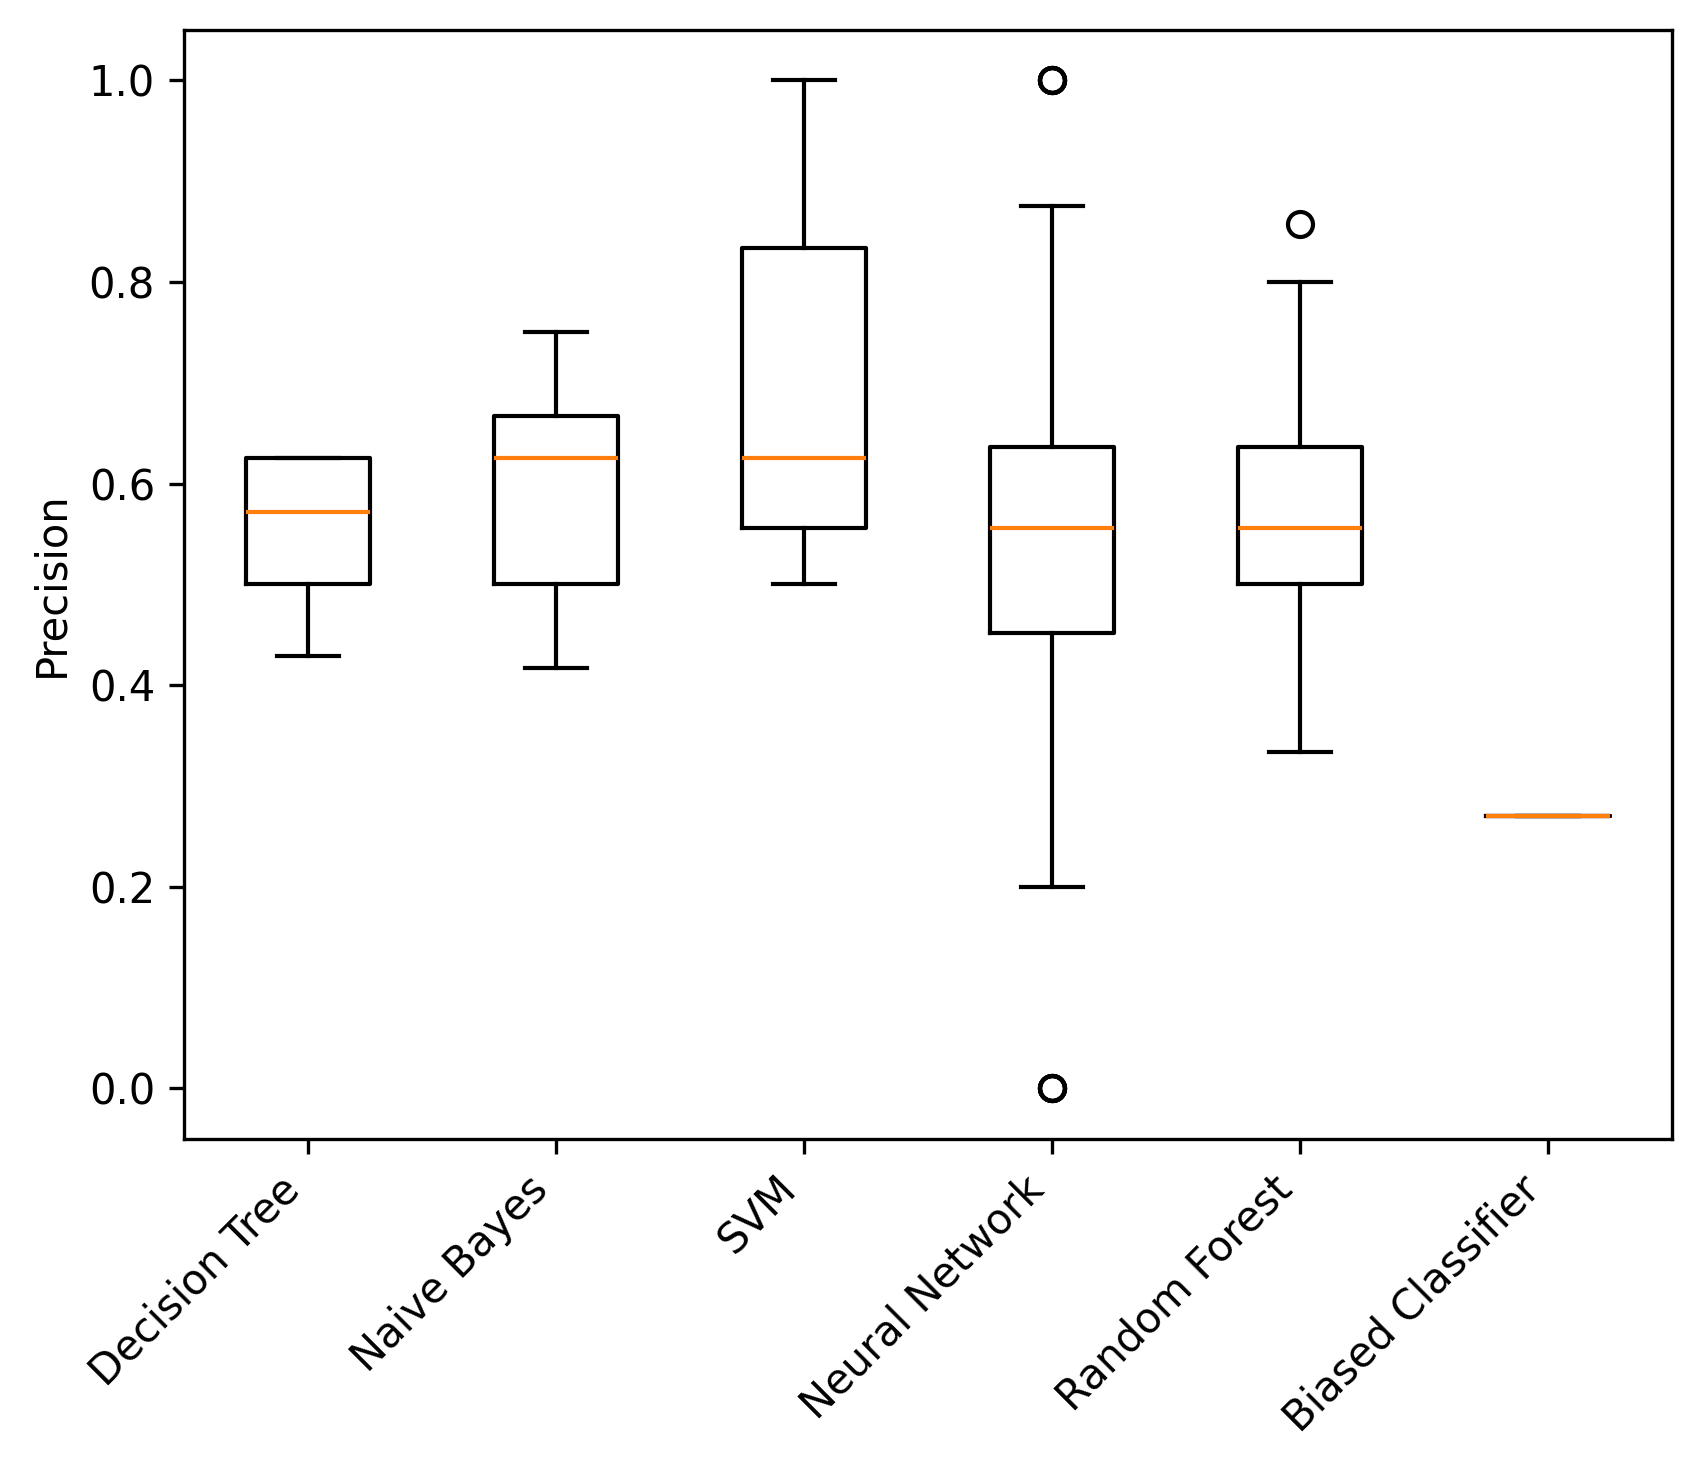
\includegraphics[width=\linewidth]{precision.png}
	      \subcaption{Precision}
	      \label{fig:precision}
	\end{minipage}
	\begin{minipage}{0.45\linewidth}
	    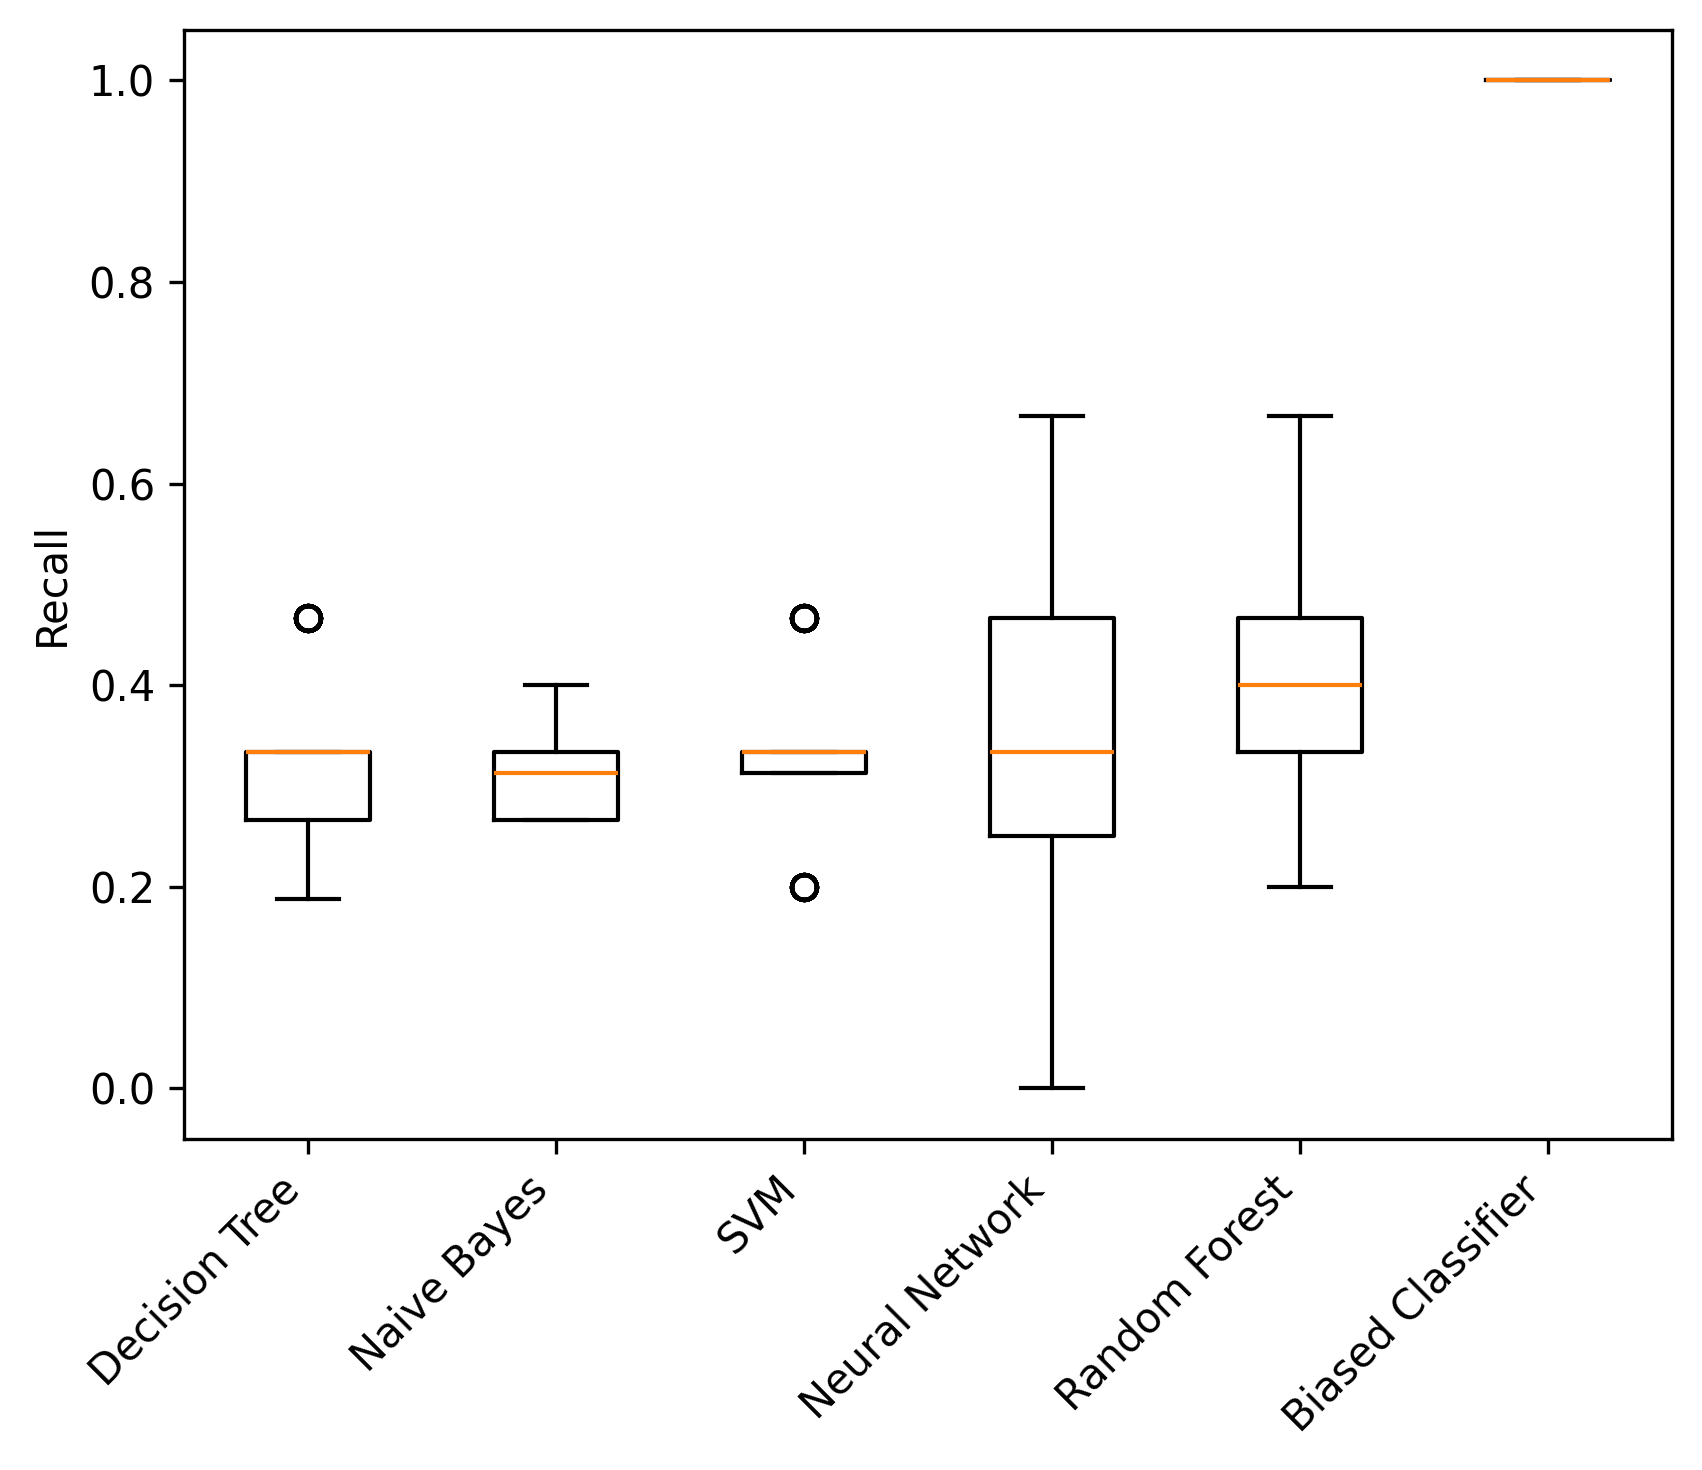
\includegraphics[width=\linewidth]{recall.png}
	    \subcaption{Recall}
	    \label{fig:recall}
        \end{minipage} \\	
	\begin{minipage}{0.45\linewidth}
	    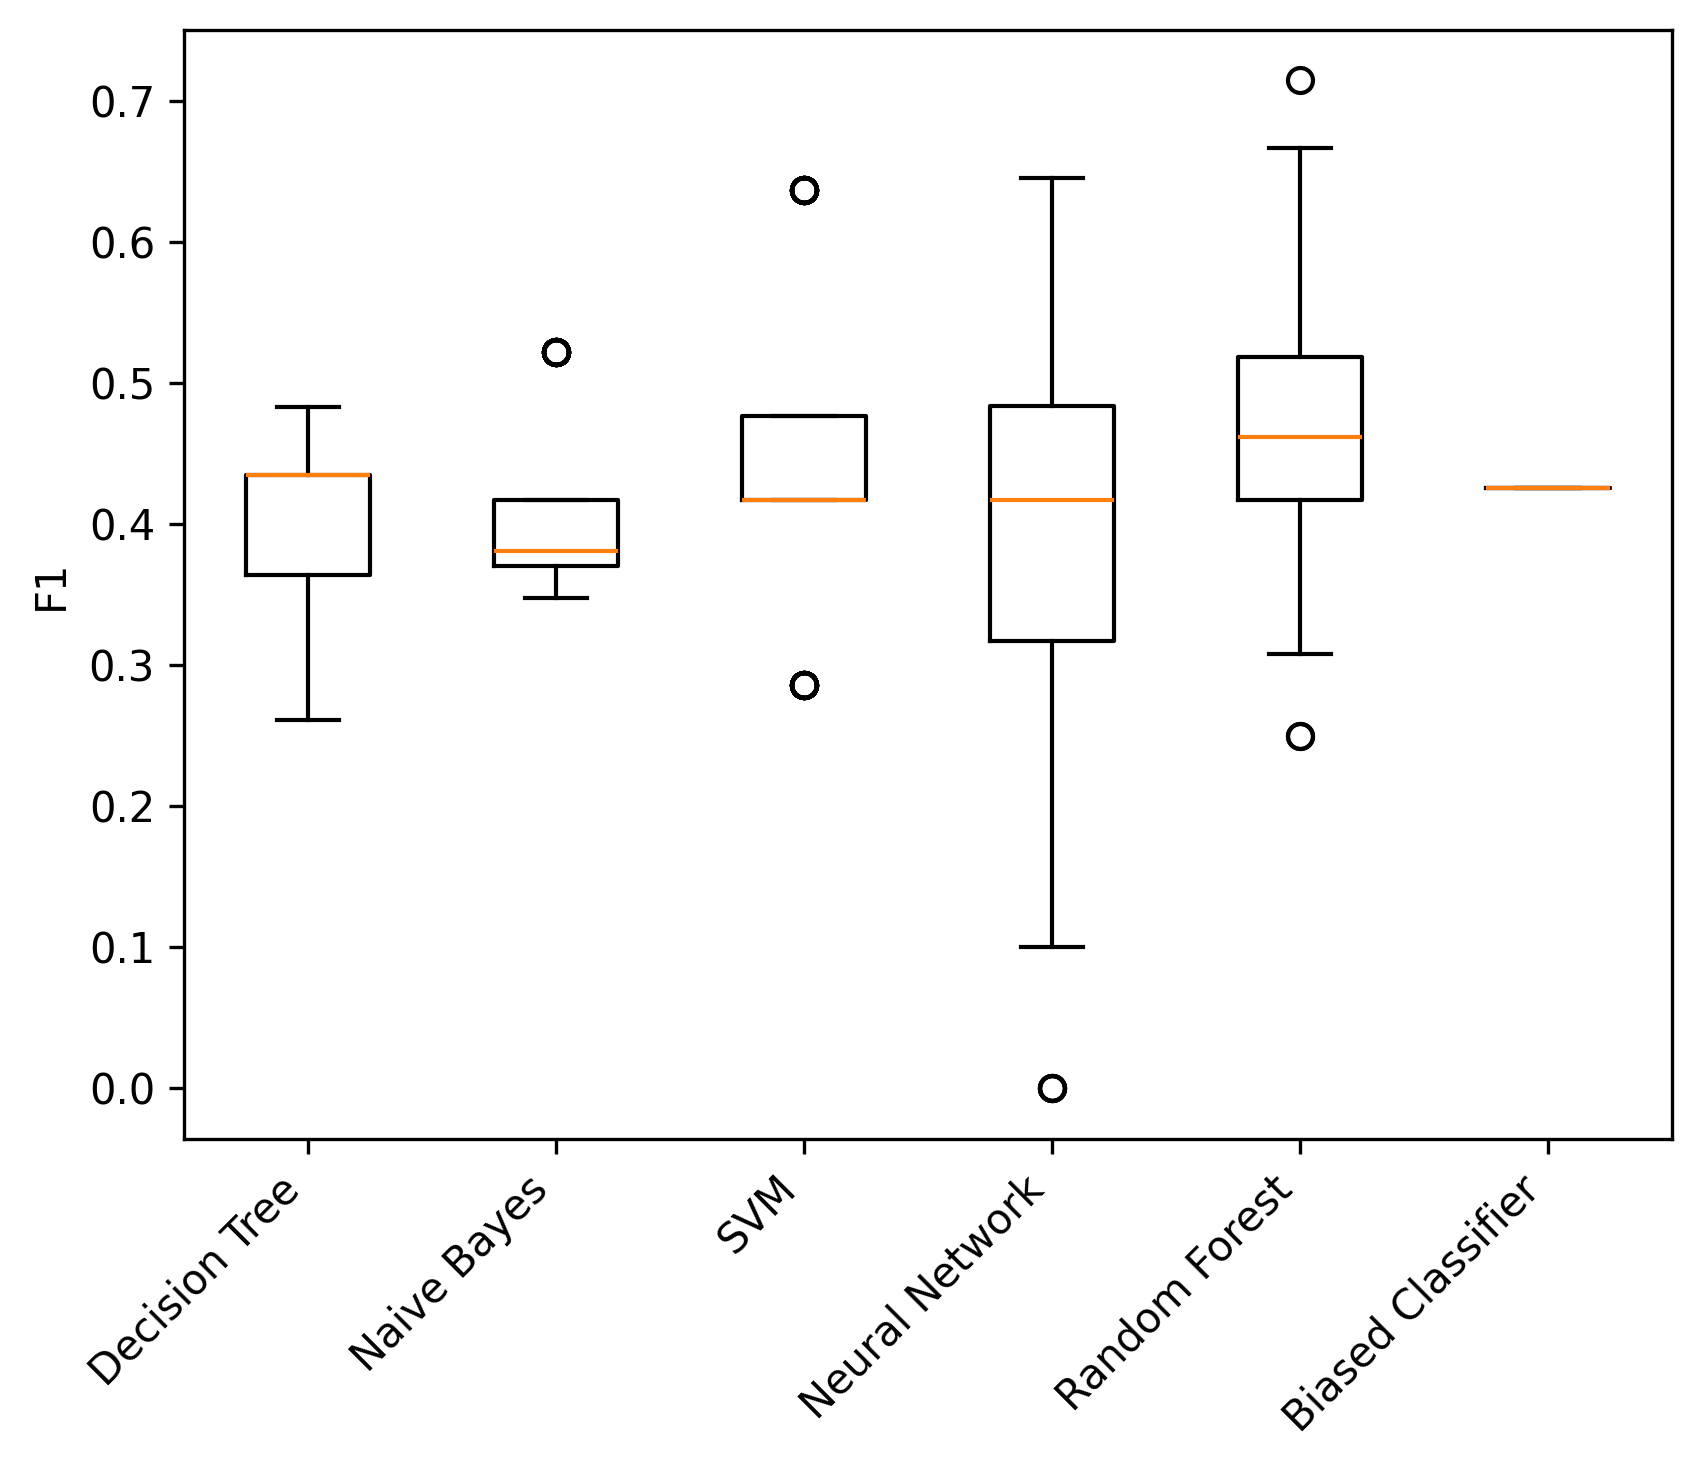
\includegraphics[width=\linewidth]{f1.png}
	    \subcaption{F1}
	\label{fig:f1}
         \end{minipage}
\caption{Boxplot showing mean and standard deviation for Precision, Recall and F1 values on all 6 classifiers (5 trained + 1 biased).}
\label{fig:boxplot}
\end{figure}


\subsection{Comparison and Significance}

% \templateInstruction{For every combination of two classifiers and every performance metric (precision, recall, f1) compare which algorithm performs better, by how much, and report the corresponding p-value in the following subsubsections:}
For every combination of two classifiers and every performance metric (precision, recall, f1) I compared which algorithm performs better, by how much, and reported the corresponding p-value. The results are as follows:
\subsubsection{F1 Values}
\begin{itemize}
    \item Mean F1 for \textbf{DT}: 0.395, Mean F1 for \textbf{NB}: 0.407 $\Rightarrow$ NB is better then DT (p-value = 0.0163).
    \item Mean F1 for \textbf{DT}: 0.395, Mean F1 for \textbf{SVM}: 0.446 $\Rightarrow$ SVM is better then DT (p-value = 0.0001).
    \item Mean F1 for \textbf{DT}: 0.395, Mean F1 for \textbf{MLP}: 0.385 $\Rightarrow$ DT is better then MLP (p-value = 0.4280).
    \item Mean F1 for \textbf{DT}: 0.395, Mean F1 for \textbf{RF}: 0.469 $\Rightarrow$ RF is better then DT (p-value = 1.1628e-07).
    \item Mean F1 for \textbf{DT}: 0.395, Mean F1 for \textbf{Biased}: 0.425 $\Rightarrow$ Biased is better then DT (p-value = 0.0156).
    \item Mean F1 for \textbf{NB}: 0.407, Mean F1 for \textbf{SVM}: 0.446 $\Rightarrow$ SVM is better then NB (p-value = 0.0001).
    \item Mean F1 for \textbf{NB}: 0.407, Mean F1 for \textbf{MLP}: 0.385 $\Rightarrow$ NB is better then MLP (p-value = 0.3585).
    \item Mean F1 for \textbf{NB}: 0.407, Mean F1 for \textbf{RF}: 0.469 $\Rightarrow$ RF is better then NB (p-value = 2.7888e-07).
    \item Mean F1 for \textbf{NB}: 0.407, Mean F1 for \textbf{Biased}: 0.425 $\Rightarrow$ Biased is better then NB (p-value = 0.0134).
    \item Mean F1 for \textbf{SVM}: 0.446, Mean F1 for \textbf{MLP}: 0.385 $\Rightarrow$ SVM is better then MLP (p-value = 0.0018).
    \item Mean F1 for \textbf{SVM}: 0.446, Mean F1 for \textbf{RF}: 0.469 $\Rightarrow$ RF is better then SVM (p-value = 0.0160).
    \item Mean F1 for \textbf{SVM}: 0.446, Mean F1 for \textbf{Biased}: 0.425 $\Rightarrow$ SVM is better then Biased (p-value = 0.3051).
    \item Mean F1 for \textbf{MLP}: 0.385, Mean F1 for \textbf{RF}: 0.469 $\Rightarrow$ RF is better then MLP (p-value = 1.8143e-06).
    \item Mean F1 for \textbf{MLP}: 0.385, Mean F1 for \textbf{Biased}: 0.425 $\Rightarrow$ Biased is better then MLP (p-value = 0.0880).
    \item Mean F1 for \textbf{RF}: 0.469, Mean F1 for \textbf{Biased}: 0.425 $\Rightarrow$ RF is better then Biased (p-value = 2.9928e-06).
\end{itemize}

\subsubsection{Precision}
\begin{itemize}
    \item Mean Precision for \textbf{DT}: 0.550, Mean Precision for \textbf{NB}: 0.591 $\Rightarrow$ NB is better then DT (p-value = 0.0017).
    \item Mean Precision for \textbf{DT}: 0.550, Mean Precision for \textbf{SVM}: 0.702 $\Rightarrow$ SVM is better then DT (p-value = 9.4202e-12).
    \item Mean Precision for \textbf{DT}: 0.550, Mean Precision for \textbf{MLP}: 0.544 $\Rightarrow$ DT is better then MLP (p-value = 0.7997).
    \item Mean Precision for \textbf{DT}: 0.550, Mean Precision for \textbf{RF}: 0.574 $\Rightarrow$ RF is better then DT (p-value = 0.0289).
    \item Mean Precision for \textbf{DT}: 0.550, Mean Precision for \textbf{Biased}: 0.270 $\Rightarrow$ DT is better then Biased (p-value = 1.6744e-18).
    \item Mean Precision for \textbf{NB}: 0.591, Mean Precision for \textbf{SVM}: 0.702 $\Rightarrow$ SVM is better then NB (p-value = 7.8212e-07).
    \item Mean Precision for \textbf{NB}: 0.591, Mean Precision for \textbf{MLP}: 0.544 $\Rightarrow$ NB is better then MLP (p-value = 0.1320).
    \item Mean Precision for \textbf{NB}: 0.591, Mean Precision for \textbf{RF}: 0.574 $\Rightarrow$ NB is better then RF (p-value = 0.3069).
    \item Mean Precision for \textbf{NB}: 0.591, Mean Precision for \textbf{Biased}: 0.270 $\Rightarrow$ NB is better then Biased (p-value = 2.6677e-18).
    \item Mean Precision for \textbf{SVM}: 0.702, Mean Precision for \textbf{MLP}: 0.544 $\Rightarrow$ SVM is better then MLP (p-value = 4.7533e-12).
    \item Mean Precision for \textbf{SVM}: 0.702, Mean Precision for \textbf{RF}: 0.574 $\Rightarrow$ SVM is better then RF (p-value = 7.1454e-12).
    \item Mean Precision for \textbf{SVM}: 0.702, Mean Precision for \textbf{Biased}: 0.270 $\Rightarrow$ SVM is better then Biased (p-value = 2.6677e-18).
    \item Mean Precision for \textbf{MLP}: 0.544, Mean Precision for \textbf{RF}: 0.574 $\Rightarrow$ RF is better then MLP (p-value = 0.1932).
    \item Mean Precision for \textbf{MLP}: 0.544, Mean Precision for \textbf{Biased}: 0.270 $\Rightarrow$ MLP is better then Biased (p-value = 2.3726e-15).
    \item Mean Precision for \textbf{RF}: 0.574, Mean Precision for \textbf{Biased}: 0.270 $\Rightarrow$ RF is better then Biased (p-value = 3.6462e-18).
\end{itemize}
\subsubsection{Recall}
\begin{itemize}
    \item Mean Recall for \textbf{DT}: 0.317, Mean Recall for \textbf{NB}: 0.315 $\Rightarrow$ DT is better then NB (p-value = 0.7397).
    \item Mean Recall for \textbf{DT}: 0.317, Mean Recall for \textbf{SVM}: 0.329 $\Rightarrow$ SVM is better then DT (p-value = 0.3100).
    \item Mean Recall for \textbf{DT}: 0.317, Mean Recall for \textbf{MLP}: 0.325 $\Rightarrow$ MLP is better then DT (p-value = 0.5862).
    \item Mean Recall for \textbf{DT}: 0.317, Mean Recall for \textbf{RF}: 0.403 $\Rightarrow$ RF is better then DT (p-value = 1.6645e-07).
    \item Mean Recall for \textbf{DT}: 0.317, Mean Recall for \textbf{Biased}: 1.000 $\Rightarrow$ Biased is better then DT (p-value = 1.6744e-18).
    \item Mean Recall for \textbf{NB}: 0.315, Mean Recall for \textbf{SVM}: 0.329 $\Rightarrow$ SVM is better then NB (p-value = 1.0000).
    \item Mean Recall for \textbf{NB}: 0.315, Mean Recall for \textbf{MLP}: 0.325 $\Rightarrow$ MLP is better then NB (p-value = 0.4060).
    \item Mean Recall for \textbf{NB}: 0.315, Mean Recall for \textbf{RF}: 0.403 $\Rightarrow$ RF is better then NB (p-value = 2.4980e-11).
    \item Mean Recall for \textbf{NB}: 0.315, Mean Recall for \textbf{Biased}: 1.000 $\Rightarrow$ Biased is better then NB (p-value = 1.6744e-18).
    \item Mean Recall for \textbf{SVM}: 0.329, Mean Recall for \textbf{MLP}: 0.325 $\Rightarrow$ SVM is better then MLP (p-value = 0.6559).
    \item Mean Recall for \textbf{SVM}: 0.329, Mean Recall for \textbf{RF}: 0.403 $\Rightarrow$ RF is better then SVM (p-value = 7.1186e-08).
    \item Mean Recall for \textbf{SVM}: 0.329, Mean Recall for \textbf{Biased}: 1.000 $\Rightarrow$ Biased is better then SVM (p-value = 1.6744e-18).
    \item Mean Recall for \textbf{MLP}: 0.325, Mean Recall for \textbf{RF}: 0.403 $\Rightarrow$ RF is better then MLP (p-value = 1.9083).
    \item Mean Recall for \textbf{MLP}: 0.325, Mean Recall for \textbf{Biased}: 1.000 $\Rightarrow$ Biased is better then MLP (p-value = 3.5552e-18).
    \item Mean Recall for \textbf{RF}: 0.403, Mean Recall for \textbf{Biased}: 1.000 $\Rightarrow$ Biased is better then RF (p-value = 2.8180e-18).
\end{itemize}
\subsection{Practical Usefulness}
% \templateInstruction{Discuss the practical usefulness of the obtained classifiers in a realistic bug
% prediction scenario (1 paragraph).}
The obtained classifiers can be used in a realistic bug prediction scenario to predict the bug prone classes in the codebase. The classifiers can be used to identify the classes that are more likely to contain bugs and hence can be used to prioritize the testing and verification of those classes. 
This can help in reducing the time and effort required for testing and verification of the codebase and can help in improving the quality of the software by identifying the bug prone classes early in the development process.

\end{document}
